%========================================
\chapter{THESIS PROPOSAL}
\label{ch:prop}
%========================================

Physics-Informed Machine Learning (PIML) is a new paradigm and hot topic of research that combines data-driven and physics-based strategies, which started with Physics-Informed Neural Networks (PINNs), and is currently being expanded by further approaches.  

This thesis aims to replace the ecRad radiation module of the Integrated Forecasting System (IFS), the operational weather and climate model of the European Centre for Medium-Range Weather Forecasts (ECMWF). Despite its influence for the atmospheric simulation, the current numerical ecRad module is very processing-demanding. Therefore, it is not usually executed for every timestep and grid point (in latitude and longitude) of the IFS model. Following the current trend in meteorological centers, it is expected to replace numerical modules that are part of the microphysics of weather and climate forecast models by AI-based implementations such as PIML-based.

In a first non-PIML attempt of the proposed thesis research, a Deep Neural Network (DNN) implementation of the gas-optical scheme of the radiation module was shown here. The original numerical code (RRTMGP) was replaced by a DNN model. The kernel of the RRTMGP scheme was written in Fortran 90, and performs a 3D linear interpolation of the optical depth of the atmosphere for the considered 2D grid point using a lookup table indexing temperatures, pressures and mixing fractions. The DNN implementation of the gas-optical scheme employed the TensorFlow library in the Python environment to perform training and validation of a neural network using a known dataset. The resulting trained model is written to disk to be used later by the Fortran 90 DNN implementation embedded in the radiation module. Performance and accuracy results were discussed, using the ecRad modules results as reference.

As already mentioned, this thesis proposes an incremental approach for the AI-based radiation module implementations, starting with DNN, followed by PINN, and then other PIMLs. The simple no-PIML DNN approach was already implemented for an example test case, as shown here, as a starting point. Further tests involving DNN-only implementations will come after, and PINN-based and other PIML-based are certainly foreseen.    
As previoulsy mentioned, the resulting future PIML-based implementation of the ecRad radiation module can be partially employed in the microphysics of the MPAS (Model for Prediction Across Scales) atmospheric model that was chosen for MONAN (Model for Ocean-laNd-Atmosphere predictioN) currently being developed by CPTEC/INPE and other Brazilian institutions.

The following workplan and schedule describe the steps/tasks envisaged in this thesis work,

%The work will also evaluate data-driven parameter discovery of PDEs by PINNs, which is a relatively recent approach that can be applied to replace some specific processing-requiring modules that are part of the physics of NMs used for climate and weather prediction.
 

%========================================
\section{Work Plan}
%========================================

\textbf{Thesis title}: Implementation of the ecRad Radiation Module Using Physics Informed Machine Learning

\textbf{Workplan tasks}:

\begin{itemize}[noitemsep,topsep=0pt]

\item \textbf{Bibliographic research}: review of the literature related to PIML.

\item \textbf{PIML radiation module}: implementation of a preliminary PINN version of the radiation module, including test of different problem instances, and comparison with the numerical model for numerical differences and computing performance.

\item \textbf{Optimization of the preliminary PINN-based radiation module}: improvement of the accuracy of the PINN model assuming the numerical radiation module as reference, and using optimization of the neural network architecture and/or of the hyperparameters.

\item \textbf{Other PIML approaches}: implementation of other PIML approaches (non PINN-based models) and comparison with the optimized PINN model.

\item \textbf{Further case studies}: use of the PIML implementations (including PINN-based models) in other case studies, with comparisons with the corresponding numerical implementations.

% \item \textbf{PIML complexity, XAI}: assessment of the computational complexity of the implemented PIML models, and Explainable Artificial Intelligence (XAI).

\item \textbf{Article submission}: submission of articles for conferences and indexed journals.

%\item \textbf{Revision}: review of the work, preparing for the final version.

\item \textbf{Thesis writing}: writing of the doctoral thesis and presentation slides.

\end{itemize}



%========================================
\section{Schedule}
%========================================

% schedule source file:
% https://docs.google.com/spreadsheets/d/1ZSLkj16o32JLDKYM6FDw3Dme9wPzY60L92erdBckwJI/edit?usp=sharing

\begin{figure}[H]\centering
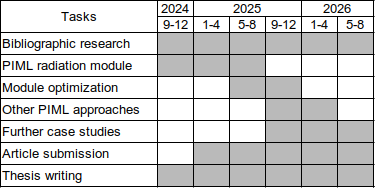
\includegraphics[width=.8\columnwidth]{schedule}
\label{fig:schedule}
\end{figure}



%========================================
\section*{Acknowledgment}
%========================================

Authors thank LNCC (National Laboratory for Scientific Computing) for grant 205341 AMPEMI (call 2020-I), which allows access to the Santos Dumont supercomputer (node of the SINAPAD, the Brazilian HPC system). This study was financed in part by the Coordination for the Improvement of Higher Education Personnel (CAPES), Brazil, finance Code 001, and also by the CNPq Project 446053/2023-6. The authors also thank the Brazilian Ministry of Science, Technology and Innovation, and the Brazilian Space Agency.